% Copyright 2004 by Till Tantau <tantau@users.sourceforge.net>.
%
% In principle, this file can be redistributed and/or modified under
% the terms of the GNU Public License, version 2.
%
% However, this file is supposed to be a template to be modified
% for your own needs. For this reason, if you use this file as a
% template and not specifically distribute it as part of a another
% package/program, I grant the extra permission to freely copy and
% modify this file as you see fit and even to delete this copyright
% notice. 

\documentclass{beamer}

% There are many different themes available for Beamer. A comprehensive
% list with examples is given here:
% http://deic.uab.es/~iblanes/beamer_gallery/index_by_theme.html
% You can uncomment the themes below if you would like to use a different
% one:
%\usetheme{AnnArbor}
%\usetheme{Antibes}
%\usetheme{Bergen}
%\usetheme{Berkeley}
%\usetheme{Berlin}
%\usetheme{Boadilla}
%\usetheme{boxes}
%\usetheme{CambridgeUS}
%\usetheme{Copenhagen}
%\usetheme{Darmstadt}
%\usetheme{default}
%\usetheme{Frankfurt}
%\usetheme{Goettingen}
%\usetheme{Hannover}
%\usetheme{Ilmenau}
%\usetheme{JuanLesPins}
%\usetheme{Luebeck}
\usetheme{Madrid}
%\usetheme{Malmoe}
%\usetheme{Marburg}
%\usetheme{Montpellier}
%\usetheme{PaloAlto}
%\usetheme{Pittsburgh}
%\usetheme{Rochester}
%\usetheme{Singapore}
%\usetheme{Szeged}
%\usetheme{Warsaw}


% Customize Warsaw color 
\setbeamercolor*{palette primary}{use=structure,fg=white,bg=red!50!black}
\setbeamercolor*{palette secondary}{use=structure,fg=white,bg=red!60!black}
\setbeamercolor*{palette tertiary}{use=structure,fg=white,bg=red!70!black}

% Customize Warsaw block title and background colors
\setbeamercolor{block title}{bg=red!50!black,fg=white}


% List your packages here

\usepackage[colorinlistoftodos]{todonotes}


\title[Progress Update]{A Generalized Open Source Platform for Building Energy Management}

% % A subtitle is optional and this may be deleted
% \subtitle{Product Proposal}

\author[B.~Lauer]{Brian~Lauer\\\and
Advisor: Dr. Suruz Miah}
% - Give the names in the same order as the appear in the paper.
% - Use the \inst{?} command only if the authors have different
%   affiliation.

\institute[Bradley University] % (optional, but mostly needed)
{
  Department of Electrical and Computer Engineering\\
  Bradley University\\
  1501 W. Bradley Avenue\\
  Peoria, IL, 61625, USA
}
% - Use the \inst command only if there are several affiliations.
% - Keep it simple, no one is interested in your street address.

\date[May~15,~2020]{Friday, May~15,~2020}
% - Either use conference name or its abbreviation.
% - Not really informative to the audience, more for people (including
%   yourself) who are reading the slides online

\logo{\hfill\href{http://www.bradley.edu}{
\includegraphics[width=0.75cm]{figs/logoBU1-Print}}}  % place logo in every page 


\subject{Mobile Robot Localization}
% This is only inserted into the PDF information catalog. Can be left
% out. 

% If you have a file called "university-logo-filename.xxx", where xxx
% is a graphic format that can be processed by latex or pdflatex,
% resp., then you can add a logo as follows:

% \pgfdeclareimage[height=0.5cm]{university-logo}{university-logo-filename}
% \logo{\pgfuseimage{university-logo}}

% Delete this, if you do not want the table of contents to pop up at
% the beginning of each subsection:
\AtBeginSubsection[]
{
  \begin{frame}<beamer>{Outline}
    \tableofcontents[currentsection,currentsubsection]
  \end{frame}
}




% Let's get started
\begin{document}

\begin{frame}
  \titlepage
\end{frame}

\begin{frame}{Outline}
  \tableofcontents
  % You might wish to add the option [pausesections]
\end{frame}

% Section and subsections will appear in the presentation overview
% and table of contents.
\section{Introduction}

\begin{frame}{Introduction}{}
  % applications of mobile robot navigation and problem description
  \begin{figure}
  	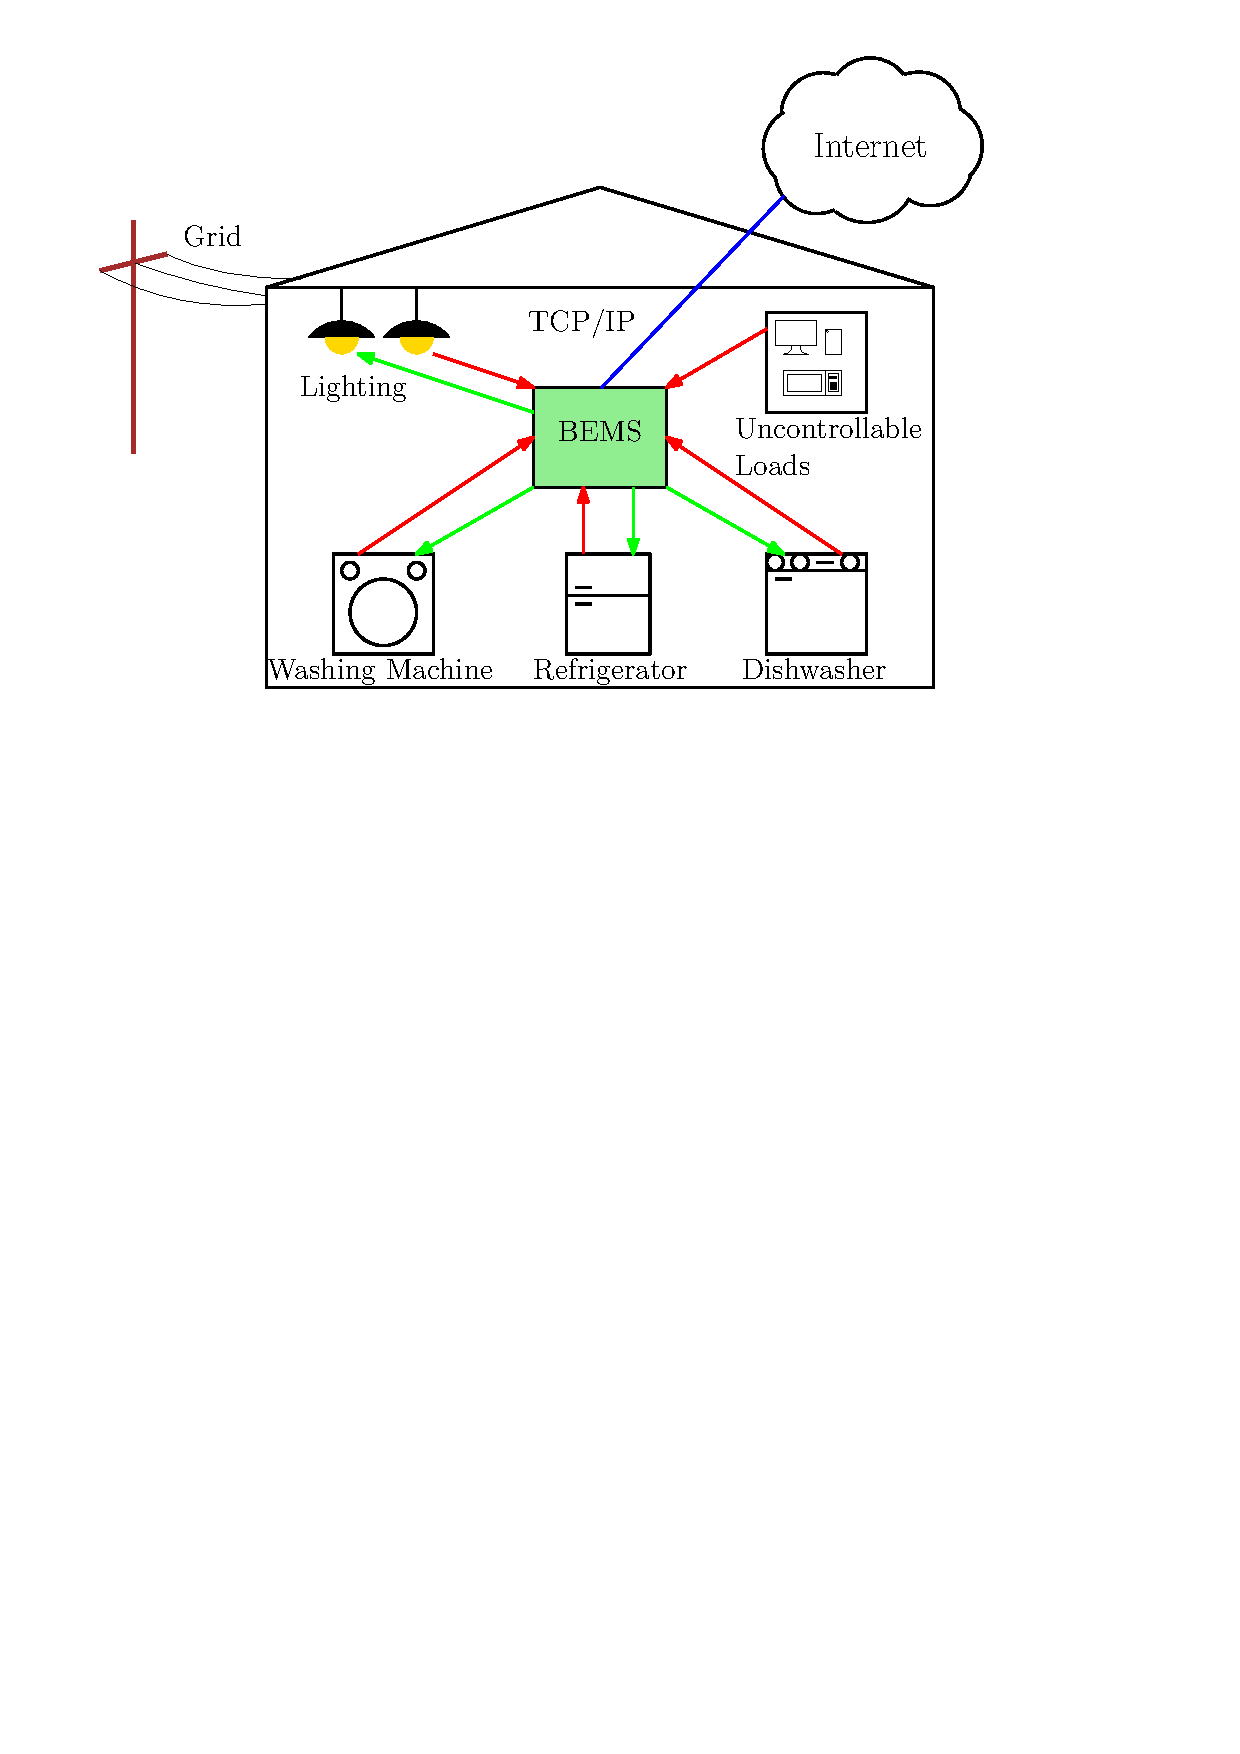
\includegraphics[scale=0.5]{figs/ipe/bemsdiagram}
  \end{figure}
\end{frame}

\begin{frame}{Introduction}{}
	\begin{figure}
		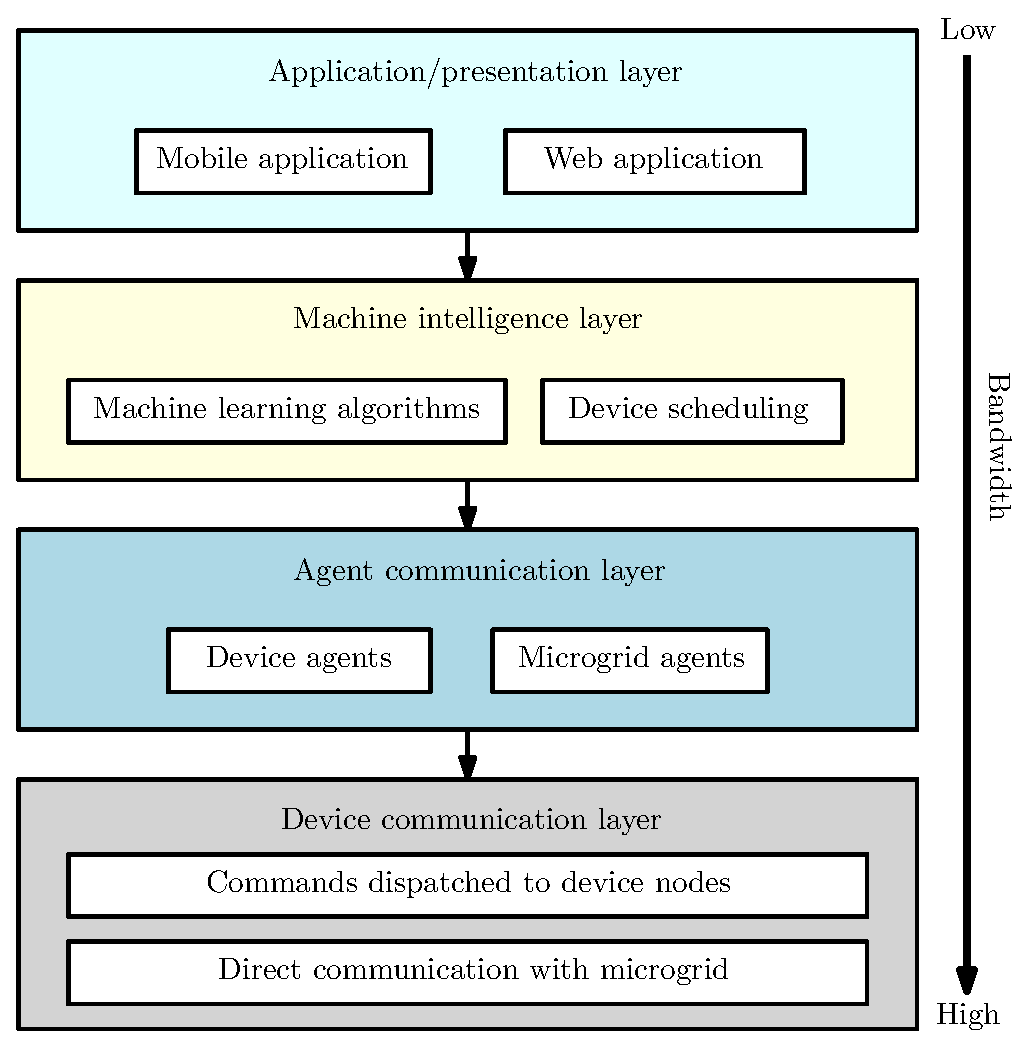
\includegraphics[scale=0.4]{figs/ipe/BEMS-softwareArchitecture}
	\end{figure}
\end{frame}

\section{Progress}
\begin{frame}{Progress}{}
	\begin{itemize}
		\item Successfully able to find device on LAN
		\item Returns URL \texttt{http://\{IP address\}:49153/setup.xml}
		\item Able to determine information like device type, manufacturer, serial number
		\item Have not fully implemented SOAP requests yet
	\end{itemize}
\end{frame}

\section{Implementation}
\begin{frame}{Implementation}{}
	\begin{itemize}
		\item Heavily based off BEMOSS Wemo API
		\item Uses SSDP to send a HTTP request over UDP to the device
		\item Responses will be returned from all UPNP devices on the network
		\item Use \texttt{if '49153/setup.xml' in header} to determine if device is a WeMo Switch
		\item \texttt{49153} is the port number and \texttt{setup.xml} is the name of the initial XML file
	\end{itemize}
\end{frame}

\begin{frame}{Implementation}{}
	\begin{itemize}
		\item Plan on use SOAP requests to retrieve and set device data 
		\item Must extract host from url
		\item In current implementation, \texttt{http://\{IP address\}:49153/setup.xml} is saved to a list
		\item Extracted URL by using pathBegin = url.rfind('/'); url = url[:pathBegin]
		\item \texttt{getState} method throwing IndexError when attempting to read from tag corresponding to \texttt{'BinaryState'}
	\end{itemize}
\end{frame}

\begin{frame}{Implementation}{}
\begin{figure}
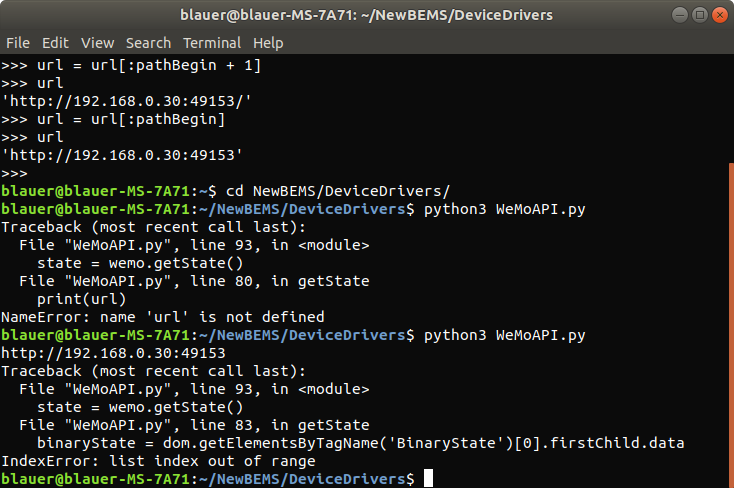
\includegraphics[scale=0.4]{figs/img/getStateIndexError}
\end{figure}
\end{frame}

\begin{frame}{Implementation}{}
	\begin{itemize}
		\item \texttt{xml.dom.minidom} used for building XML tree of tags from XML file
		\item \texttt{requests} for sending SOAP requests to device
		\item \texttt{urllib.request} for opening XML dom
	\end{itemize}
\end{frame}

\section{Plans}
\begin{frame}{Plans}{}
	\begin{itemize}
		\item Finish up adding SOAP requests to WeMo Switch API
		\item Add support in UI for Switch
		\item Look into Jemdoc and how to create a wiki with this markup language
	\end{itemize}
\end{frame}
%----------------------------------





% All of the following is optional and typically not needed. 
\appendix
\section<presentation>*{\appendixname}
\subsection<presentation>*{For Further Reading}

\begin{frame}[allowframebreaks]
  \frametitle<presentation>{For Further Reading}
    
  \begin{thebibliography}{10}
    
  \setbeamertemplate{bibliography item}[online]
  
  \bibitem{BEMOSSWiki}
  BEMOSS WeMo API
  \newblock \texttt{https://github.com/bemoss/BEMOSS3.5/wiki/API-WeMo}
  \end{thebibliography}
\end{frame}

\end{document}



%%% Local Variables:
%%% mode: latex
%%% TeX-master: t
%%% End:
